\chapter{Introduction}
\label{cha:introduction}

As a part of the \emph{Computer Systems II} lecture, this lab deals with the 
application and driver development for the System-on-Chip (SoC) kit \emph{SpartanMC}, 
which allows the design of an SoC on a FPGA target.
In particular, the task is to generate a system configuration and develop firmware
which allow distance measurements with an ultrasound sensor, a processing of the
measured data, and the view of these results on a connected OLED display. This document
reports about the implementation of the described tasks, and offers insights into the 
development processes. 

The report is structured as following. First, the functions to be implemented are summarized.
Afterwards, the toolchain use is reviewed. Then, 
the generated SoC structure is presented, and the implementations for the utilized 
subsystems are discussed. Before the report is closed with an evaluation of the work, 
a short view on the additional tasks is taken.
\subsubsection{Task Summary}
\label{subsubsec:taskSummary}

As a result of this lab, a SoC system which 
\begin{itemize}
    \item can measure a distance with an ultrasound sensor,
    \item processes the measured data to extinct wrong values and
    \item can display the data on an connected OLED Display.
\end{itemize}

shall be developed. Among the required steps are:
\begin{itemize}
\item Configuring the SoC hardware, including the peripherals for sensor and display 
connections,
\item development of drivers for the SPI and I2C Master,
\item implementation of the protocols of the ultrasound sensor and the OLED display 
driver,
\item design and implementation of a filtering algorithm for  the sensor data and
\item integration of these sub-components into a running system.
\end{itemize}


\section{SpartanMC Toolchain}
\label{sec:spartanMCToolchain}

Developing applications with a SpartanMC system requires the use of the SpartanMC
toolchain. This is a set of applications which must be executed in order to define
the system architecture, develop the firmware and execute it on the hardware. In general,
all tools are triggered by a \emph{make} target in a central makefile; that way, all 
dependency constraints are met. The main tools for the developer are:

\begin{itemize}
\item \textbf{JConfig} \hfill \\
JConfig is a graphical tool to create a new system configuration and add components to
the system. In this task, the used components are a SpartanMC soft core, a clock 
generator, and peripherals conencted to an Advanced Peripheral Bus (APB). More details 
on the system architecture are dscribed in section \ref{sec:systemArchitecture}. 
After the creation of a system configuration, it must be saved. \\
\item \textbf{System Builder} \hfill \\
The SpartanMC System Builder is invoked with the make target \emph{make all program}, 
and reads in the previously designed configuration. It builds the HDL description
of the system, triggers the synthesis of the hardware description, and flashes the 
resulting FPGA configuration onto the target board. As the synthesis and implementation
have to be performed for each system individually, this step requires some time in the
range of seconds to minutes. As long as the hardware is not changed (i.e. no change in 
JConfig), the System Builder does not need to be run again. \\
\item \textbf{Programming the FPGA} \hfill \\
With \emph{make program}, the synthesized hardware design is flashed to the FPGA, as it
is also described in the previous section. Even if the system configuration does not
change, it may be necessary to re-program the FPGA, for example if the FPGA board was 
shut down; the configuration is lost in that case. Although \emph{make program} also writes the
firmware to the memory, this step is further described in the next section.\\
\item \textbf{Programming the Processor} \hfill \\
So far, only hardware is generated. In order to program the processor with the written 
firmware, the code must be compiled, linked and assembled, and be loaded into the memory
of the system. Therefore, the compiler toolchain must be invoked. It compiles the user code
placed in \texttt{firmware/src} and \texttt{firmware/include}, and links it with the 
general libraries wihtin the SpartanMC environment. With \emph{make updateRam program},
the generated executable is transmitted to the memory of the system. The CPU core is 
resetted, and the execution of the user code starts. The target \emph{updateRam} prohibits
the hardware re-configuration and avoids the time-consuming reprogramming process for 
the FPGA target.\\
\item \textbf{Other Tools}\hfill \\
Other than the steps described previously, a serial terminal on the host pc and a logic
analyzer are used. With the serial terminal, status messages and data from the program
can be displayed; additionally, parameters can be sent to the SoC. The logic analyzer 
is helpful to debug electrical problems and can be attached to pins on the target or the 
connected peripherals.
\end{itemize}

As one can see, the central design steps are the configuration of the system architecture
with \emph{JConfig} and writing the user code as \emph{C} code.

\section{System Architecture}
\label{sec:systemArchitecture}
The SoC configuration consists of two major parts: the main system with the cpu core 
and the peripherals. 

For this task, the main system may consist only of one SpartanMC soft core, a memory
block, and a clock generator. This is the minimum configuration, and offers a low complexity.

In order to implement the functions described in the task summary, the SoC requires four 
peripherals: a UART Light Peripheral for serial communication to the host PC, a SPI master 
to send data and commands to the display, an I$^{2}$C master to read out the sensor, 
and a General-Purpose I/O Port, requried to reset the display. These are included in the 
system configuration, as shown in Fig. \ref{fig:SystemArchitecture}.

\begin{figure}
    \centering
    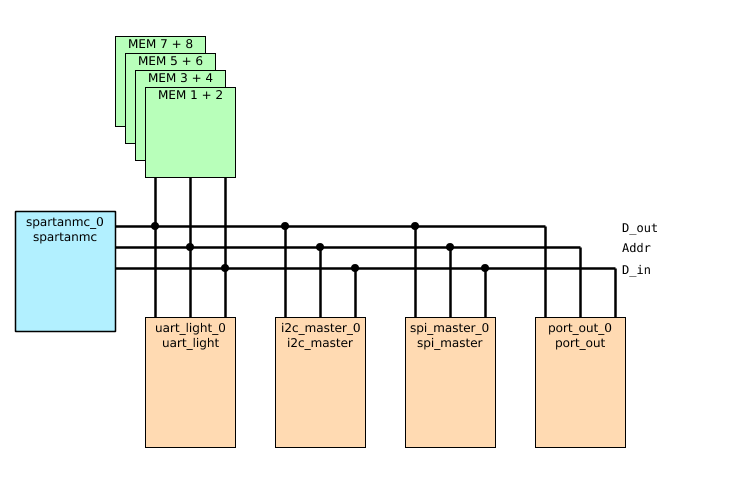
\includegraphics[width=0.9\textwidth]{images/SystemOverview.png}
    \label{fig:SystemArchitecture}
    \caption{System Architecture for the SoC.}
\end{figure}

\section{General Code Structure}
\label{sec:generalCodeStructure}
As a result to this task, several files of C sourcecode have been created. These 
can be split into application code and driver functionality.

The application code consists of the main function (in \texttt{main.c}), which calls
the initializing functions for all modules, and the filter (in \texttt{filter.c/filter.h}).
In the main loop, which is repeated forever, the functions to read the sensor value,
filter it and send it to the display and the host processor are called.

The driver functionality created in this lab is separated into ultrasound sensor reading
procedures (\texttt{ultrasound.c}), SPI sending and init procedures (\texttt{spi.c}), and 
GPIO and I$^{2}$C procedures (\texttt{gpio.c, i2c.c}). The display functions are implemented
in \texttt{oled25664.c}, while a header for this given file had to be added manually.

As presented above, the code structure follows the typical approach for microcontrollers:
first, all peripherals and modules are initialized; in the main loop, abstract driver 
functions are used, so that the concerns for each task are separated.